\documentclass[12pt]{article}

\usepackage{pablo-devoir}
%\usepackage{pablo-listings}
\usepackage[a5paper,margin=1cm]{geometry}

\pagestyle{empty}

\title{Fonctions Statistiques}
\date{14/01/15}
\classe{2\up{des}14}
\dsnum{DS 4}

\begin{document}
\maketitle

\begin{exercice}[Fonctions affines]~
  On considère deux fonctions $f:x\mapsto -0,5x+6$, et $g:x\mapsto 2x-4$,
  définies sur l'ensemble des réels $\mathbb{R}$.
  \begin{enumerate}
    \item \emph{Donner les variations de $f$ et $g$ sur leur ensemble de définition.} La fonction $f$ est affine, de coefficient directeur $-0,5$ : elle est décroissante. La fonction $g$ est affine, de coefficient directeur $2$ : elle est croissante.
    \item \emph{Calculer $f(4)$ et $g(4)$.}
      \begin{multicols}{2}
      \begin{align*}
        f(4) &= -0,5\times 4+6 \\
             &= -2 + 6 \\
             &= 4
      \end{align*}

      \begin{align*}
        g(4) &= 2\times 4-4 \\
             &= 8 -4 \\
             &= 4
      \end{align*}
    \end{multicols}
    \item \emph{Comparer, sans nouveaux calculs, $f(10)$ et $g(10)$.} Puisque $f$ est décroissante, $f(10)\leq f(4)$. Puisque $g$ est croissante, $g(10)\geq g(4)$. Enfin, puisque $f(4)=g(4)$, $f(10)\leq g(10)$.
  \end{enumerate}
\end{exercice}

\begin{exercice}[Compétition]
  Voici les scores obtenus dans une compétition de tir à l'arc par
  les 40 joueuses.

  \begin{tabular}{c||c|c|c|c|c|c|c|c|c|c}
    Score
    & 400
    & 410
    & 433
    & 442
    & 453
    & 460
    & 478
    & 483
    & 492
    & 498
    \\
    \hline
    Effectif
    & 2
    & 4
    & 2
    & 8
    & 5
    & 7
    & 5
    & 4
    & 1
    & 2
    \\
    \hline
    ECC
    & 2
    & 4
    & 8
    & 16
    & 21
    & 28
    & 33
    & 37
    & 38
    & 40
  \end{tabular}

  \begin{enumerate}
    \item \emph{Calculer la médiane et les quartiles de cette série.}
      On calcule les effectifs cumulés croissants (ECC) dans le tableau.

      \begin{enumerate}
        \item Il y a 40 valeurs, qui est un nombre pair, donc la médiane est la valeur entre la 20\up{e} et 21\up{e} valeur, soit 453.
        \item Le premier quartile $Q_1$ est la plus petite valeur supérieure à un quart des valeurs, c'est-à-dire 10. C'est donc 442.
        \item Le troisième quartile $Q_3$ est la plus petite valeur supérieure à trois quart des valeurs, soit 30. C'est donc 478.
      \end{enumerate}
  \item \emph{L'an passé, la moitié des candidates avait obtenu un score inférieur à
    440. À l'aide de cette seule information, peut-on dire que le niveau des
  joueuses a plutôt augmenté ou plutôt baissé ?}
  Cela signifie que la médiane l'an passé était égale à 440. La médiane a donc augmenté : le niveau a plutôt augmenté.
  \end{enumerate}

\end{exercice}

\begin{exercice}[Échantillonnage]~
  \noindent\emph{Les deux questions sont indépendantes.}

  \emph{Travaillant dans un laboratoire de contrôle pharmaceutique, vous êtes chargé(e) d'étudier deux traitements $A$ et $B$, censés guérir une certaine maladie. On sait que pour cette maladie, 30\% des malades guérissent spontanément (c'est-à-dire sans médicament) en moins d'une semaine. La question à laquelle vous devez répondre est : Ces médicaments permettent-ils une guérison plus rapide ?}

  \begin{enumerate}
    \item \emph{Testé auprès de 30 personnes, le traitement $A$ en a guéri 17 en moins d'une semaine. On note $p_A$ la proportion théorique de malades guérissant en moins d'une semaine avec le médicament $A$.}
      \begin{enumerate}
        \item \emph{Déterminer un intervalle de confiance à 95~\% de $p_A$, donné par la formule $\left[f-\frac{1}{\sqrt{n}};f+\frac{1}{\sqrt{n}}\right]$, où $f$ est la fréquence des guérisons de l'échantillon en moins d'une semaine, et $n$ la taille de l'échantillon.}

          L'échantillon est composé de 30 personnes, et la fréquence de guérison en moins d'une semaine dans cet échantillon est $\dfrac{17}{30}$. Donc l'intervalle de confiance est $\left[ \frac{17}{30}-\frac{1}{\sqrt{30}};\frac{17}{30}+\frac{1}{\sqrt{30}}  \right]$, c'est-à-dire environ $\left[ 0,38;0,75 \right]$.
        \item \emph{Pouvez-vous affirmer que ce médicament accélère le temps de guérison ? Justifier.} Sans médicament, 30~\% des malades guérissent en moins d'une semaine. Ce nombre est hors de l'intervalle de confiance, donc on peut affirmer sans trop de chances de se tromper que $p_A$ est supérieure à 0,30, c'est-à-dire que le médicament $A$ est efficace.
      \end{enumerate}
    \item \emph{Un intervalle de confiance à 95~\% de la proportion $p_B$ de guérisons en moins d'une semaine avec le traitement $B$ est $\left[0,27;0,41\right]$. Pouvez-vous affirmer que ce traitement accélère la guérison ? Justifier.}
      Cette fois-ci, $30\%$ est compris dans l'intervalle, donc on ne peut pas affirmer que $p_B$ soit supérieure à 30\% : rien ne prouve que le médicament $B$ soit efficace.
  \end{enumerate}
\end{exercice}

\begin{exercice}[Résolution graphique d'(in)équations]
  On considère les fonctions $f$ et $g$, définies sur $\left[ -4;6 \right]$ et
  représentées sur le graphique suivant.
  \begin{center}
    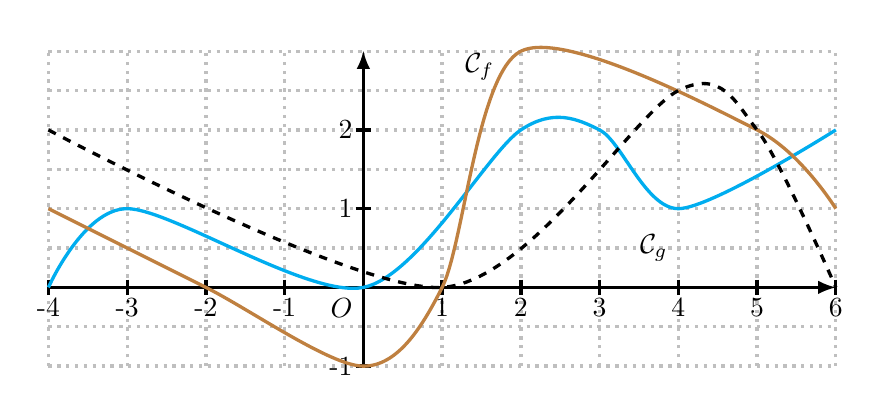
\begin{tikzpicture}[very thick,xscale=1, yscale=1]
      \draw[dotted, lightgray, xstep=1, ystep=.5] (-4, -1) grid (6, 3);
      \draw[-latex] (-4,0) -- (6,0);
      \draw[-latex] (0,-1) -- (0,3);
      \foreach \x in {-4, -3, -2, -1, 1, 2, 3, 4, 5, 6} {
        \draw (\x,0) node[below]{\x};
        \draw (\x,{0.1}) -- (\x,{-0.1});
      }
      \foreach \y in {-1, 1, 2} {
        \draw (0,\y) node[left]{\y};
        \draw (-.1, \y) -- (.1, \y);
      }
      \draw [cyan] plot [smooth, tension=0.5] coordinates {
        (-4,0)
        (-3, 1.0)
        (0, 0)
        (2, 2)
        (3, 2)
        (4, 1)
        (6, 2)
      };
      \draw [brown] plot [smooth, tension=0.5] coordinates {
        (-4,1)
        (-2, 0)
        (0, -1.0)
        (1, 0)
        (2, 3)
        (5, 2)
        (6, 1)
      };
      \draw [dashed] plot [smooth, tension=0.5] coordinates {
        (-4,2)
        (1, 0)
        (4, 2.5)
        (5, 2)
        (6,0)
      };
      \draw (0,0) node[below left]{$O$};
      \draw (1.8, 2.8) node[left]{$\mathcal{C}_f$};
      \draw (4.0, 0.5) node[left]{$\mathcal{C}_g$};
    \end{tikzpicture}
  \end{center}
  \emph{Répondre aux questions par lecture graphique.}
  \begin{enumerate}
    \item \emph{Déterminer les solutions de $f(x)<0$} La courbe de $f$ est située en dessous de l'axe des abscisses pour $x\in\left] -2;1 \right[$.
    \item \emph{Déterminer les solutions de $f(x)\geq g(x)$.} Les solutions sont les abscisses des points de $f$ situés au dessus des points de $g$, c'est-à-dire $\left[-4;-3,5 \right]\cup\left[1,3;5,5 \right]$.
    \item \emph{Tracer la courbe d'une fonction $h$ telle que les solutions de $h(x)>f(x)$ soient $\left[ -4;1 \right[ \cup \left] 4;5 \right[$.} Voir l'exemple en pointillés.
      \item \emph{Pourquoi n'existe-t-il pas de fonction $p$ telle $p(x) \geq g(x)$, et $p(x)\leq0$ sur $\left[ 2;4 \right]$ ?} Prenons par exemple $x=3$. Puisque $p(x)\leq0$, alors $p(3)\leq0$. Donc $p(3)$ est négatif. Mais $p(3)\geq g(3)$, et $g(3)>0$. Donc $p(3)$ est à la fois négatif et strictement positif : c'est impossible.
  \end{enumerate}

\end{exercice}

\begin{exercice}[Moyenne]
  \emph{Un élève a une moyenne de 9 à trois devoirs. Quelle note minimale devra-t-il avoir au prochain devoir pour que sa moyenne soit au moins égale à 10 ?} La note minimale que cet élève peut avoir est telle que sa moyenne soit égale à 10. Appelons $x$ cette note. Elle vérifie :

  \[\frac{3\times9+x}{4}=10\]

  Et la solution de cette équation est $x=13$.
\end{exercice}

\end{document}
